A user can request a runtime switch between synchronization protocols. A typical use case is when a significant slowdown is observed or memory usage reaches a certain treshold. The simulation engine will swap out the current kernels with new instances while preserving the state of the models and the simulation itself, and resume using the new synchronization protocol. There is no real limit on the number of switches, but the replacing and synchronizing of the kernels comes at a runtime cost that is dependent on the number of present kernels and the actual hardware the simulation runs on. In a test case with 2 kernels the overhead of a double runtime switch is less than a second.
This is an experimental but promising feature that can be used in an automated framework driven by machine learning techniques.

%TODO combination with statistics gathering
Dxex optionally collects runtime statistics for each kernel. These record any measurable event in the simulation such as : events created/destroyed, inter/intra kernel event frequency, reverts, GVT calculations, lookahead and eot values and insights into the fairness between the kernels themselves. Using this information it is possible to detect an imbalance between the simulation rounds that a single kernel executes compared to dependent or influencing kernels, observe how balanced inter kernel message traffic actually is during a simulation or measure reverted transitions in optimistic synchronization.
The same information can, as in the visualization tool, be used programmatically to extend dxex with visualization software that shows the simulation from a white box perspective or provide feedback to drive synchronization switching.

The same information can, as in the visualization tool, be used programmatically to extend dxex with visualization software that shows the simulation from a white box perspective or provide feedback to drive synchronization switching.
Figures \ref{fig:pholdtree_visualize_seq},\ref{fig:pholdtree_visualize_parDFS},\ref{fig:pholdtree_visualize_parBFS} give an example of the modular visualization output generated by dxex after simulation the PholdTree model. These figures demonstrate the effect of allocation visually and show the high inter kernels event count that degrades performance, as we will demonstrate in
\nameref{PholdTreeallocation} . Dotted lines represent connections between models where no events were exchanged, directed edges represents events with frequency as weight, coloring is used to distinguish inter versus intra kernel events.
% Add figure
\begin{figure}
    \center
    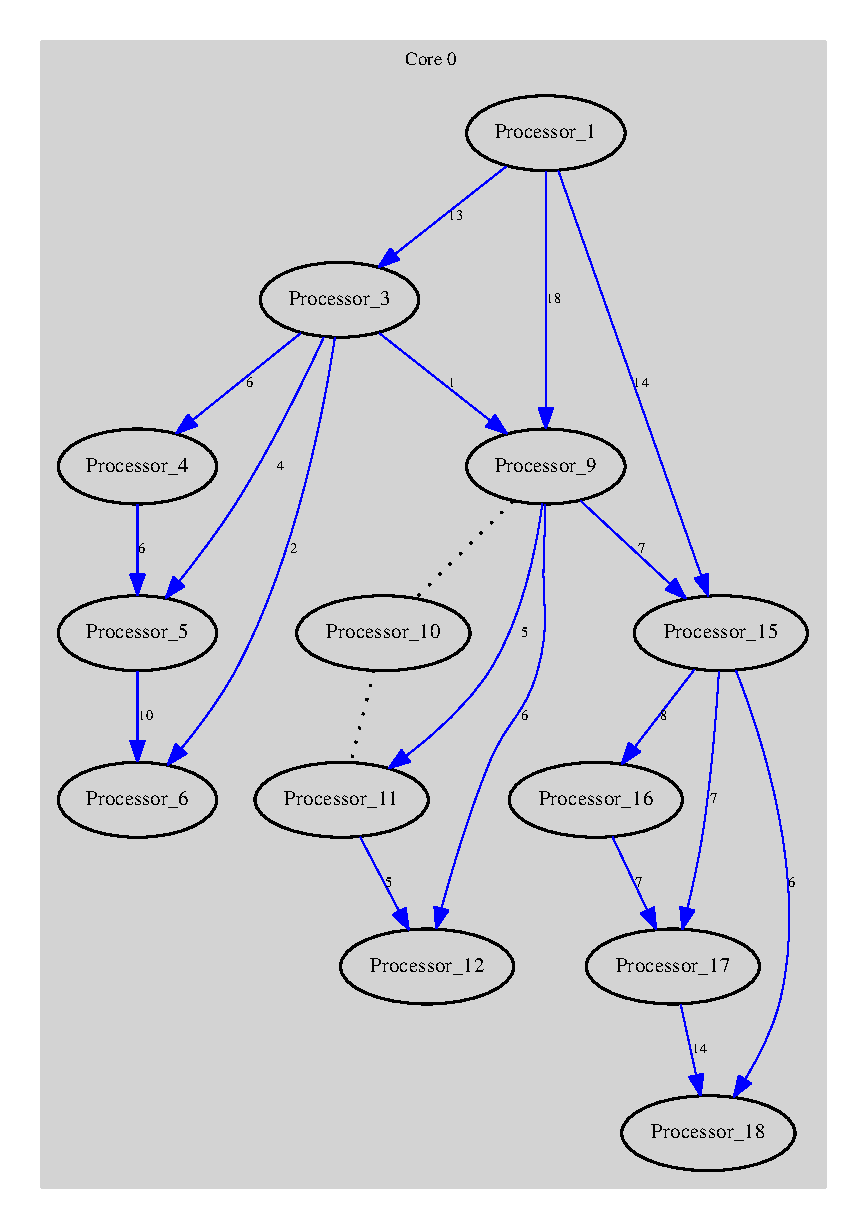
\includegraphics[width=\plotfraction\columnwidth, height=6cm, keepaspectratio]{fig/pholdtreed1n3t5000.eps}
    \caption{Visualization of PholdTree (d=1,n=3,t=5000) sequential simulation.}
    \label{fig:pholdtree_visualize_seq}
\end{figure}
\begin{figure}
    \center
    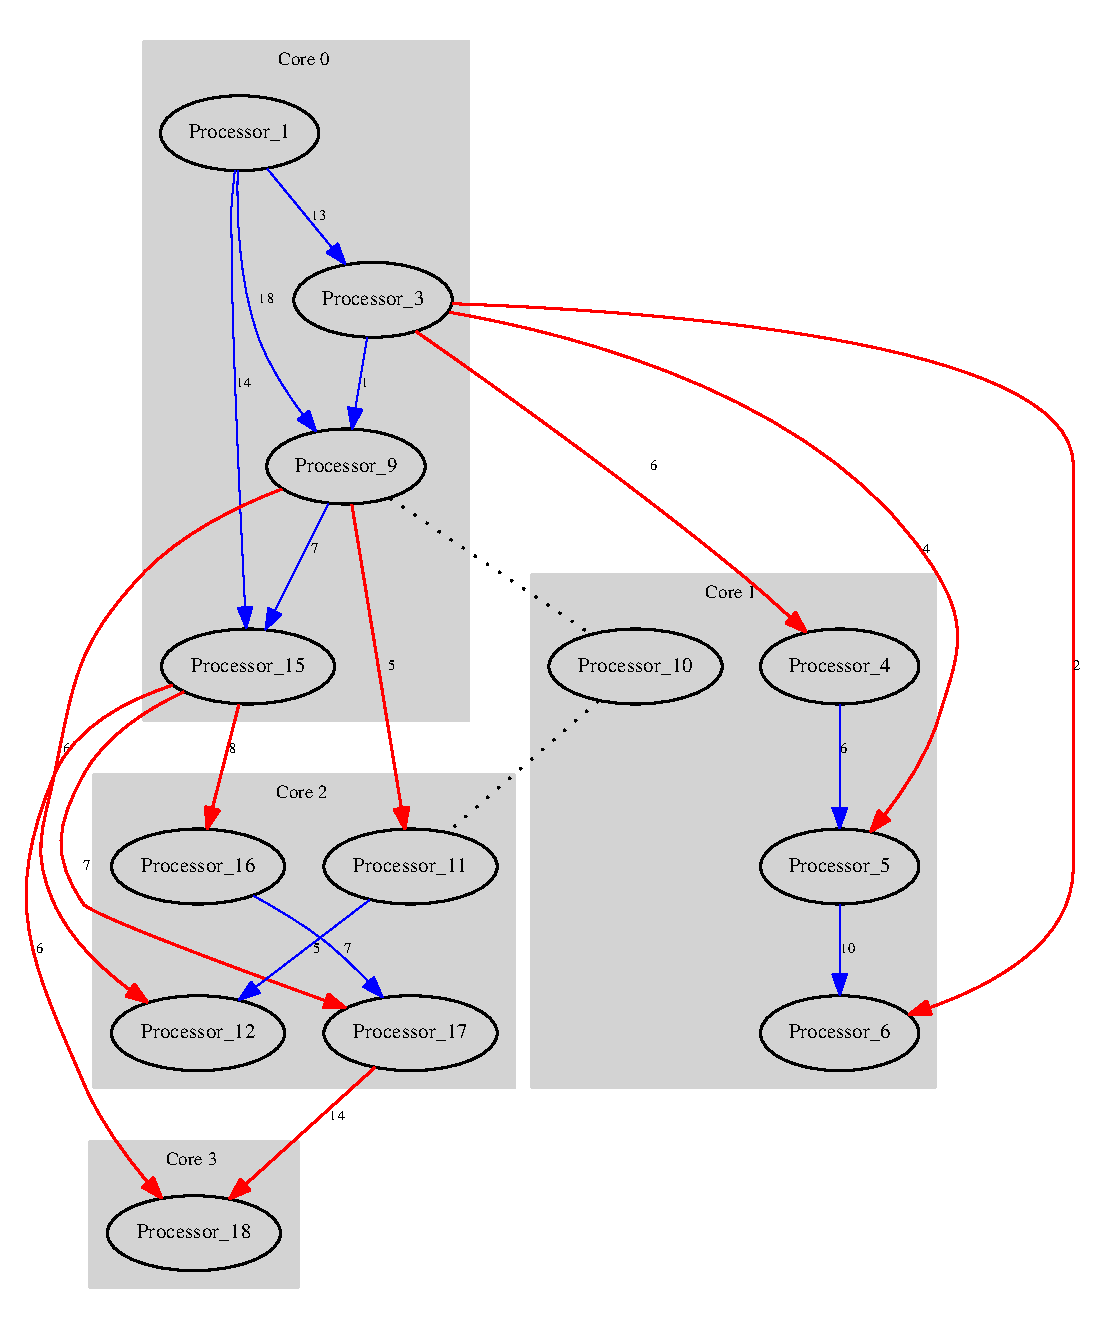
\includegraphics[width=\plotfraction\columnwidth,  height=6cm, keepaspectratio]{fig/pholdtreed1n3t5000c4BFS.eps}
    \caption{Visualization of PholdTree (d=1,n=3,t=5000) parallel simulation with breadth first allocation and 4 kernels.}
    \label{fig:pholdtree_visualize_parBFS}
\end{figure}
\begin{figure}
    \center
    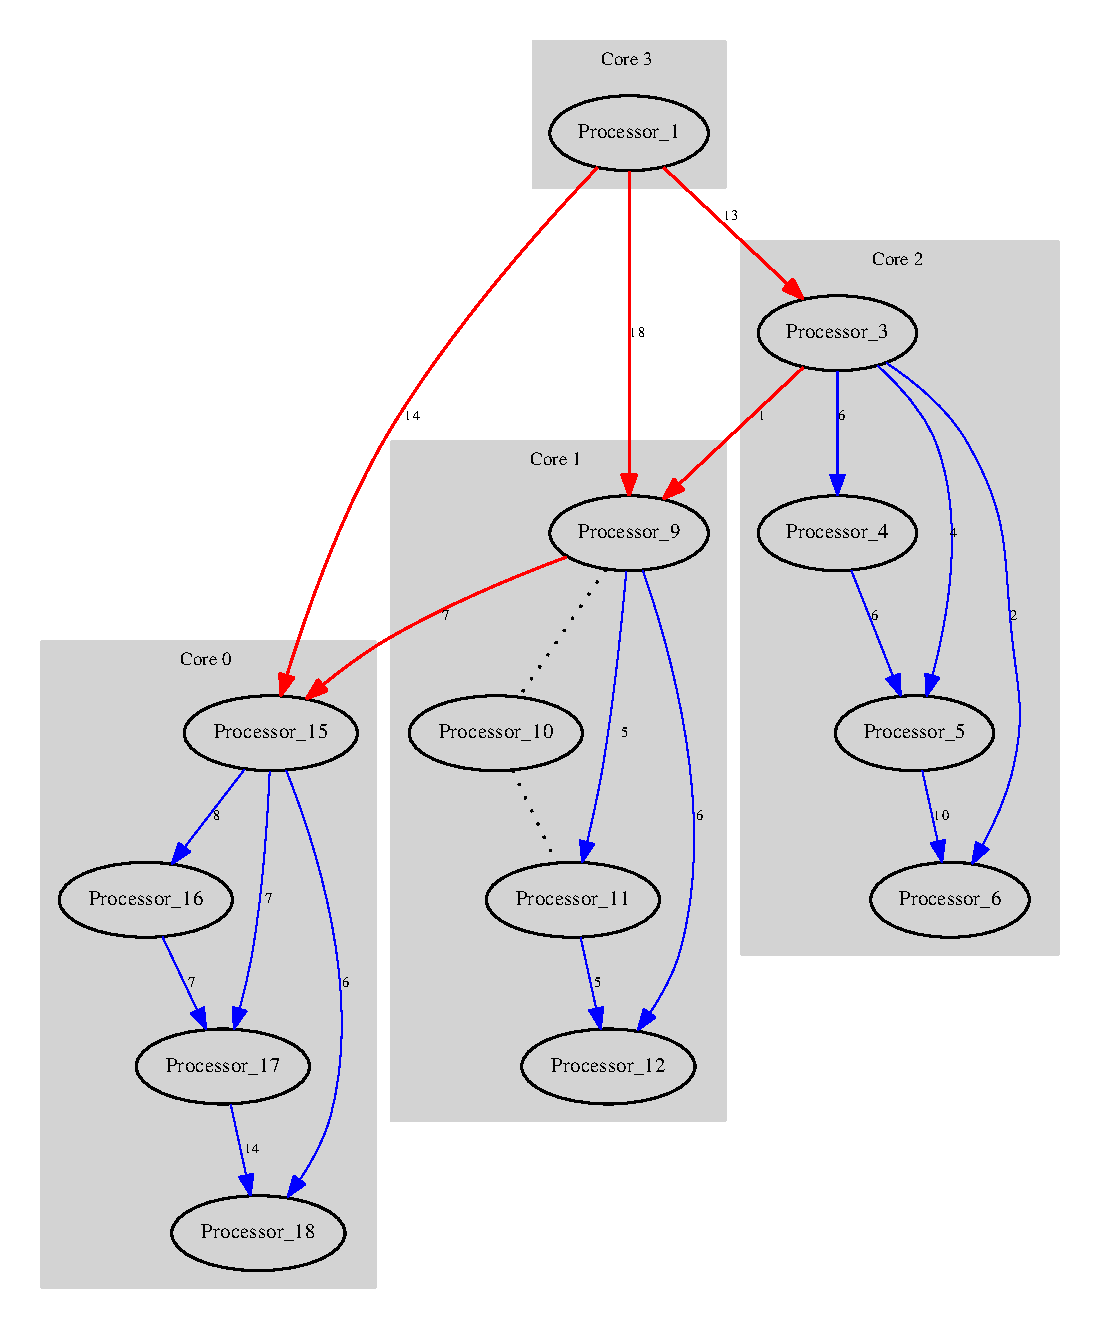
\includegraphics[width=\plotfraction\columnwidth,  height=6cm, keepaspectratio]{fig/pholdtreed1n3t5000c4DFS.eps}
    \caption{Visualization of PholdTree (d=1,n=3,t=5000) parallel simulation with depth first allocation and 4 kernels.}
    \label{fig:pholdtree_visualize_parDFS}
\end{figure}
